\documentclass[12pt,a4paper,oneside]{article}
\usepackage[a4paper,left=3cm,right=2cm,top=2.5cm,bottom=2.5cm]{geometry}
\usepackage{graphicx}
\graphicspath{{img/}}
\usepackage{verbatim}
\usepackage{listings}
\usepackage{color}
\usepackage{caption}
\usepackage{float}


\begin{document}
\author{Valent\'{i}n Korenblit}
\title{\vspace{-2cm} LLVM/Clang integration to Buildroot
\\ Internship progress report}
\maketitle

\section*{Summary}
The main purpose of the internship is to integrate LLVM/Clang packages to Buildroot.
This would activate new functionalities such as enabling llvmpipe software rast
erizer (useful for systems which do not have a dedicated GPU) and providing OpenCL
support for existing packages already present in Buildroot (OpenCV, Mesa3D). Once
LLVM is present on the system, new packages that make use of this infrastructure
can be added to Buildroot.\\
Once this part of the project is achieved, the next step is to create a cross-toolchain
based on Clang to compile Buildroot componentes supported by this front-end.
\footnote{Mainline Linux kernel and glibc do not yet compile with Clang}

\section*{State of the project}
After some research concerning the state of the art of the LLVM project, the objectives
of the internship were presented and discussed at the Buildroot Developers Meeting
in Brussels \footnote{https://elinux.org/Buildroot:DeveloperDaysFOSDEM2018}, obtaining
the following conclusions:
\begin{itemize}
  \item LLVM itself is very useful for other packages (Mesa3D's llvmpipe or OpenJDK's
        Jit compiler).
  \item It is questionable whether there is a need for Clang in Buildroot, as GCC
        is still needed and it has mostly caught up with Clang regarding performance,
        diagnostics and static analysis. It would be possible to build a complete
        userspace but some packages may break.
  \item LLVM does not have a stable API between major releases, so only these releases
        can be used.
  \item It could be useful to have a host-clang package that is user selectable.
  \item The long-term goal is to have a complete clang-based toolchain.
\end{itemize}

The first patch series aims only to activate LLVM support for Mesa3D, and is divided
into these 3 patches:
\begin{itemize}
  \item package/llvm: new host package
  \item package/llvm: enable target variant
  \item package/mesa3d: enable llvm support
\end{itemize}

It must be considered that with respect to the RFC series,
\footnote{http://lists.busybox.net/pipermail/buildroot/2017-July/196163.html}
AMDGPU target support was removed and it will be added once it can be tested. Currently,
the supported targets are X86, ARM and AArch64, and llvm.mk ensures that only
the necessary targets are built.

\subsection*{Considerations}

\subsubsection*{LLVM makefile}
In order to cross-compile LLVM for the target, llvm-config and llvm-tblgen tools
must be installed on the host. In the first patch series, a minimal version of
host-llvm containing only these two tools is provided. To do this, most of the
{\fontfamily{qcr}\selectfont HOST\_LLVM\_CONF\_OPTS} are set to OFF. However,
this does not avoid building LLVM libraries, what takes around one hour in a
recent machine. To prevent this and build only the necessary tools:\\
{\fontfamily{qcr}\selectfont HOST\_LLVM\_MAKE\_OPTS = llvm-tblgen llvm-config}\\

Things to be considered when cross-compiling LLVM:
\begin{itemize}
  \item Path to host's llvm-tblgen: {\fontfamily{qcr}\selectfont
  -DLLVM\_TABLEGEN}
  \item Must specify that it is a cross-compilation: {\fontfamily{qcr}\selectfont
  -DCMAKE\_CROSSCOMPILING}
  \item Default target triple: {\fontfamily{qcr}\selectfont
  -DLLVM\_DEFAULT\_TARGET\_TRIPLE}
  \item Host triple (native code generation for the target): {\fontfamily{qcr}\selectfont
  -DLLVM\_HOST\_TRIPLE}
  \item Target architecture: {\fontfamily{qcr}\selectfont
  -DLLVM\_HOST\_TRIPLE}
  \item Targets to build: {\fontfamily{qcr}\selectfont
  -DLLVM\_TARGETS\_TO\_BUILD}
\end{itemize}

The result of the compilation will be one shared library containing all LLVM
libraries called libLLVM.so, as {\fontfamily{qcr}\selectfont
-DLLVM\_BUILD\_LLVM\_DYLIB} is set to ON.\\

One important step in the process is the fact of replacing llvm-config in STAGING\_DIR
by its host variant. This is because llvm-config compiled for the target cannot
run on the host, and this is needed to build applications that use LLVM, as it
prints the compiler flags, linker flags and object libraries needed to link
against LLVM.

\subsubsection*{Mesa3D}

Currently, Mesa3D is linking against LLVM libraries statically. When setting the
option {\fontfamily{qcr}\selectfont MESA3D\_CONF\_OPTS += --enable-llvm-shared-libs},
the build fails because it cannot find LLVM libraries. Apparently, the problem is
that llvm-config placed in STAGING\_DIR is not working properly, as it provides
the following outputs to this commands:
\begin{itemize}
  \item {\fontfamily{qcr}\selectfont./llvm-config --shared-mode\\
        static}
  \item {\fontfamily{qcr}\selectfont./llvm-config --link-shared\\
        llvm-config: error: libLLVM-5.0.so is missing}

  \item {\fontfamily{qcr}\selectfont./llvm-config --libnames\\
        libLLVMLTO.a libLLVMPasses.a libLLVMObjCARCOpts.a...}
\end{itemize}

Even if llvm-config returns the correct lib directory, it assumes it has to use
LLVM static libraries, and as the configure script from Mesa3D calls llvm-config
--link-shared --libs (in case --enable-shared-libs is activated) the build
will fail. Mesa's configure script clearly states that llvm-config may not give
the correct output when LLVM is build as a single shared library.


\subsection*{Achievements}

At this date, llvmpipe was successfully tested in the following systems:

\begin{itemize}
  \item x86\_64
  \item ARM
  \item AArch64
\end{itemize}

\subsubsection*{x86\_64}
The tests for x86\_64 were done using an AMD A4-3300M microprocessor. The built
system uses a Linux kernel 4.9, X window system and works correctly with OpenGL.
During this test it was possible to appreciate the better performance provided by
llvmpipe with respect to softpipe.
\begin{figure}[H]
\centering
  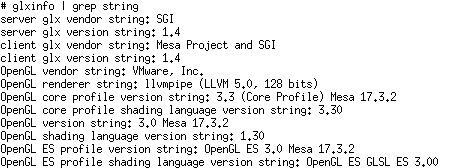
\includegraphics[scale=0.75]{img/llvmpipe-glspecs.png}
  \caption{OpenGL specs}
  \label{fig:llvmpipe-glspecs}
\end{figure}

Some benchmarks were run to compare llvmpipe against the classic softpipe software
rasterizer and the AMD Radeon HD6480. Table \ref{tab:glmark2_x86} shows how much
the LLVM code optimizer improves the performance for rendering:

\begin{table}[h!]
  \begin{center}
    \caption{Results of GLMark2 and GLMark2-es2 benchmarks for x86_64}
    \label{tab:glmark2_x86}
    \begin{tabular}{ c |c c }
    & {GLMark2} & {GLMark2-es2} \\
    \hline
    Radeon HD6480 & 156 & 156 \\
    llvmpipe & 47 & 52 \\
    softpipe & 3 & 3 \\
    \end{tabular}
  \end{center}
\end{table}


\subsubsection*{ARM}
In order to test LLVM for ARM architecture, Raspberry Pi 2 and Raspberry Pi 3
development boards were used. For the case of the Raspberry Pi 3, the 32-bit
defconfig was selected.

\begin{table}[h!]
  \begin{center}
    \caption{Raspberry Pi 2 and 3 Hardware Specifications}
    \label{tab:rpi_specs}
    \begin{tabular}{c c c c c }
    Board & Family & SoC & CPU & GPU \\
    \hline
    RPi 2 & BCM2709 & BCM2836 @ 900 MHz & ARMv7 Cortex-A7 (Quad Core) & VC4 \\
    RPi 3 & BCM2710 & BCM2837 @ 1.2 GHz & ARMv8 Cortex-A53 (Quad Core) & VC4 \\
    \end{tabular}
  \end{center}
\end{table}

Raspberry supports only OpenGL ES, so only GLMark2-es2 could be tested. When
trying to execute {\fontfamily{qcr}\selectfont glmark2} the following errors are
obtained:\\\\
{\fontfamily{qcr}\selectfont Error: GLX version >= 1.3 is required}\\\\
{\fontfamily{qcr}\selectfont Error: Error: Couldn't get GL visual config}\\\\
{\fontfamily{qcr}\selectfont Error: main: Could not initalize canvas}\\\\


\begin{table}[h!]
  \begin{center}
    \caption{Results of GLMark2-es2 for ARM}
    \label{tab:glmark2_ARM}
    \begin{tabular}{c|c}
    & {GLMark2-es2} \\
    \hline
    RPi2 softpipe & 0\\
    Rpi2 llvmpipe & 0\\
    Rpi3 (32-bit) softpipe & 0\\
    Rpi3 (32-bit) llvmpipe & 11\\
    \end{tabular}
  \end{center}
\end{table}

Table \ref{tab:glmark2_ARM} shows an improvement in rendering when LLVM is used,
and also the higher computing power of the Cortex-A53 microprocessor.

\subsubsection*{AArch64}
Buildroot offers a defconfig to install a 64-bit system on the Raspberry Pi 3
(raspberrypi3\_64\_defconfig). There is a little improvement in rendering with
respect to the 32-bit version:

\begin{table}[h!]
  \begin{center}
    \caption{Results of GLMark2-es2 for AArch64}
    \label{tab:glmark2_AArch64}
    \begin{tabular}{c|c}
    & {GLMark2-es2} \\
    \hline
    Rpi3 (64-bit) softpipe & 0\\
    Rpi3 (64-bit) llvmpipe & 13\\
    \end{tabular}
  \end{center}
\end{table}

\subsection*{Considerations}
\begin{itemize}
    \item By default, the defconfigs for Raspberry Pi present in Buildroot have
    /dev management set to {\fontfamily{qcr}\selectfont Dynamic using devtmps only}.
    This must be changed to {\fontfamily{qcr}\selectfont Dynamic using devtmps +
    eudev} in order to allow Linux kernel to load modules dyamically, such as the
    VC4 device driver.

    \item To load VC4 device driver, assuming that the {\fontfamily{qcr}\selectfont
    \boot} partition has the {\fontfamily{qcr}\selectfont overlays/} directory with
    its dtbo files inside, the next options must be configured:
    \begin{itemize}
      \item Add cma=256M to cmdline.txt
      \item Set gpu\_mem/gpu\_mem\_1024 to 256 in config.txt
      \item Add dtoverlay=vc4-kms-v3d to config.txt
    \end{itemize}

    This steps allow to load the VC4 driver correctly, however it is not yet
    working well with X. When trying to execute any {\fontfamily{qcr}\selectfont
    glx} command, such as {\fontfamily{qcr}\selectfont glxinfo} or
    {\fontfamily{qcr}\selectfont glxgears}, it returns the following error:\\\\
    {\fontfamily{qcr}\selectfont Error: couldn't find RGB GLX visual or fbconfig}

    Possible causes:
    \begin{itemize}
      \item Mesa is not installing libglx.so in {\fontfamily{qcr}\selectfont
      /usr/lib/xorg/modules/extensions/}.
      \item Mesa3D package in Buildroot states that a vanilla kernel 4.5+ must
      be used with Gallium VC4 (defconfig uses kernel from raspberrypi's Github).
      However, even in this case or using Eric Anholt's kernel\footnote{ https://
      github.com/anholt/mesa/wiki/VC4-complete-Raspbian-upgrade} the error persists.
    \end{itemize}


\end {itemize}

\subsection*{Next steps}
\begin{itemize}
  \item Enable dynamic linking for Mesa3D. This is important because when building
        packages that link against LLVM libraries the same problem may arise.
  \item For Raspberry Pi:
    \begin{itemize}
      \item Activate glx.
      \item Activate OpenGL for VC4.
    \end{itemize}
  \item Prepare next patch series:
  \begin{itemize}
    \item Provide an option to install full host-llvm.
    \item Activate OpenCL.
    \item Activate Clang (needs full host-llvm installed).
    \item Add support for more targets.
  \end{itemize}
\end{itemize}

\end{document}
